% ======================================================================
% common-fontsize-en.tex
% Copyright (c) Markus Kohm, 2001-2022
%
% This file is part of the LaTeX2e KOMA-Script bundle.
%
% This work may be distributed and/or modified under the conditions of
% the LaTeX Project Public License, version 1.3c of the license.
% The latest version of this license is in
%   http://www.latex-project.org/lppl.txt
% and version 1.3c or later is part of all distributions of LaTeX 
% version 2005/12/01 or later and of this work.
%
% This work has the LPPL maintenance status "author-maintained".
%
% The Current Maintainer and author of this work is Markus Kohm.
%
% This work consists of all files listed in MANIFEST.md.
% ======================================================================
%
% Paragraphs that are common for several chapters of the KOMA-Script guide
% Maintained by Markus Kohm
%
% ======================================================================

\KOMAProvidesFile{common-fontsize-en.tex}
                 [$Date: 2022-10-06 14:30:20 +0200 (Do, 06. Okt 2022) $
                  KOMA-Script guide (common paragraphs: fontsize)]
\translator{Markus Kohm\and Krickette Murabayashi\and Karl Hagen}

\section{Choosing the Document Font Size}
\seclabel{fontOptions}%
\BeginIndexGroup
\BeginIndex{}{font>size}%

\IfThisCommonFirstRun{%
  The main font and its size are central elements in the design of a document.
  As stated in \autoref{cha:typearea}, the division of the page into the text
  area and the margins fundamentally depends on them. The main font is the one
  that is used for most of the text in a document. All variations, whether in
  shape, thickness, slant, or size, are related to the main font.%
}{%
  The information in \autoref{sec:\ThisCommonFirstLabelBase.fontOptions}
  applies equally to
  \IfThisCommonLabelBase{scrlttr2}{\Class{scrlttr2}\OnlyAt{scrlttr2}}%
  {this chapter}. \IfThisCommonLabelBase{scrlttr2}{By contrast, the
    \Package{scrletter} package by itself does not offer font-size selection
    but depends completely on the class you use.}{} So if you have already
  read and understood \autoref{sec:\ThisCommonFirstLabelBase.fontOptions}, you
  can \IfThisCommonLabelBase{scrlttr2}{continue to
    \autopageref{sec:\ThisCommonLabelBase.fontOptions.end} at the end of this
    section. If you use \Package{scrletter}, you can }{}%
  skip directly to \autoref{sec:\ThisCommonLabelBase.fontOptions.next},
  \autopageref{sec:\ThisCommonLabelBase.fontOptions.next}.%
}

\begin{Declaration}
  \OptionVName{fontsize}{size}
\end{Declaration}
While\IfThisCommonLabelBase{scrlttr2}{\OnlyAt{\Class{scrlttr2}}}{%
  \textnote{\KOMAScript{} vs. standard classes}} the standard classes support
only a very limited number of font sizes,
\IfThisCommonLabelBase{scrlttr2}{\Class{scrlttr2}}{\KOMAScript} provides the
ability to specify any \PName{size} for the main font. You can also use any
known \TeX unit as a unit for the \PName{size}. If the \PName{size} is
specified without a unit, it is assumed to be \PValue{pt}.\iffree{}{ The exact
  procedure for setting the font size is documented for experts and interested
  users in \autoref{sec:maincls-experts.addInfos},
  \DescPageRef{maincls-experts.option.fontsize}.}

If you set the option within the document, the main font size and the
dependent font sizes of the commands \Macro{tiny}, \Macro{scriptsize},
\Macro{footnotesize}, \Macro{small}, \Macro{normalsize}, \Macro{large},
\Macro{Large}, \Macro{LARGE}, \Macro{huge} and \Macro{Huge} are changed.  This
can be useful, for example, if you want %
\IfThisCommonLabelBase{scrlttr2}{another letter }{the appendix }%
to be set in a smaller font size.

Note\textnote{Attention!} that using this option after
\IfThisCommonLabelBase{scrextend}{potentially loading
  \hyperref[cha:typearea]{\Package{typearea}}\IndexPackage{typearea}%
  \important{\hyperref[cha:typearea]{\Package{typearea}}}}{loading the class}
does not automatically recalculate the type area and margins (see
\DescRef{typearea.cmd.recalctypearea}\IndexCmd{recalctypearea},
\autoref{sec:typearea.typearea},
\DescPageRef{typearea.cmd.recalctypearea}). However, if this recalculation is
performed, it will be based on the current main font size. The effects of
changing the main font size upon other loaded packages or the class used
depends on these packages and on the class.  \IfThisCommonLabelBase{maincls}{%
  This means that you can encounter errors which are not the fault of
  \KOMAScript, and even the \KOMAScript{} classes themselves do not
  recalculate all lengths if the main font size changes after loading the
  class.%
}{%
  \IfThisCommonLabelBase{scrlttr2}{%
    You can encounter errors which are not the fault of \KOMAScript{}, and
    further, the \Class{scrlttr2} class itself does not recalculate all
    lengths if the main font size changes after loading the class.%
  }{%
    This means that you can encounter errors which are not the fault of
    \KOMAScript{}.%
  }%
}%

This\textnote{Attention!} option should by no means be misinterpreted as a
substitute for \Macro{fontsize} (see \cite{latex:fntguide}). Also, you should
not use it in place of one of the font size commands that are relative to the
main font, from \Macro{tiny} to \Macro{Huge}. The use within a paragraph is
therefore also explicitly prohibited.
\IfThisCommonLabelBase{scrlttr2}{%
  For \Class{scrlttr2} the default is \OptionValue{fontsize}{12pt}.

  \begin{Example}
    \phantomsection\label{sec:\ThisCommonLabelBase.fontOptions.end}%
    Suppose the organization in the sample letter is the \emph{``Friends of
      Noxious Font Sizes''}, for which reason it should be set in 14\Unit{pt}
    instead of 12\Unit{pt}. You can achieve this by making a small change to
    the first line:%
    \lstinputcode[xleftmargin=1em]{letter-example-06-en.tex}%
    Alternatively, the option could be set as an optional argument to
    \DescRef{\LabelBase.env.letter}:
    \lstinputcode[xleftmargin=1em]{letter-example-05-en.tex}%
    Since the text area is not recalculated in this late change of the font
    size, the two results differ in \autoref{fig:scrlttr2.letter-05-06}.
    \begin{figure}
      \centering
      \frame{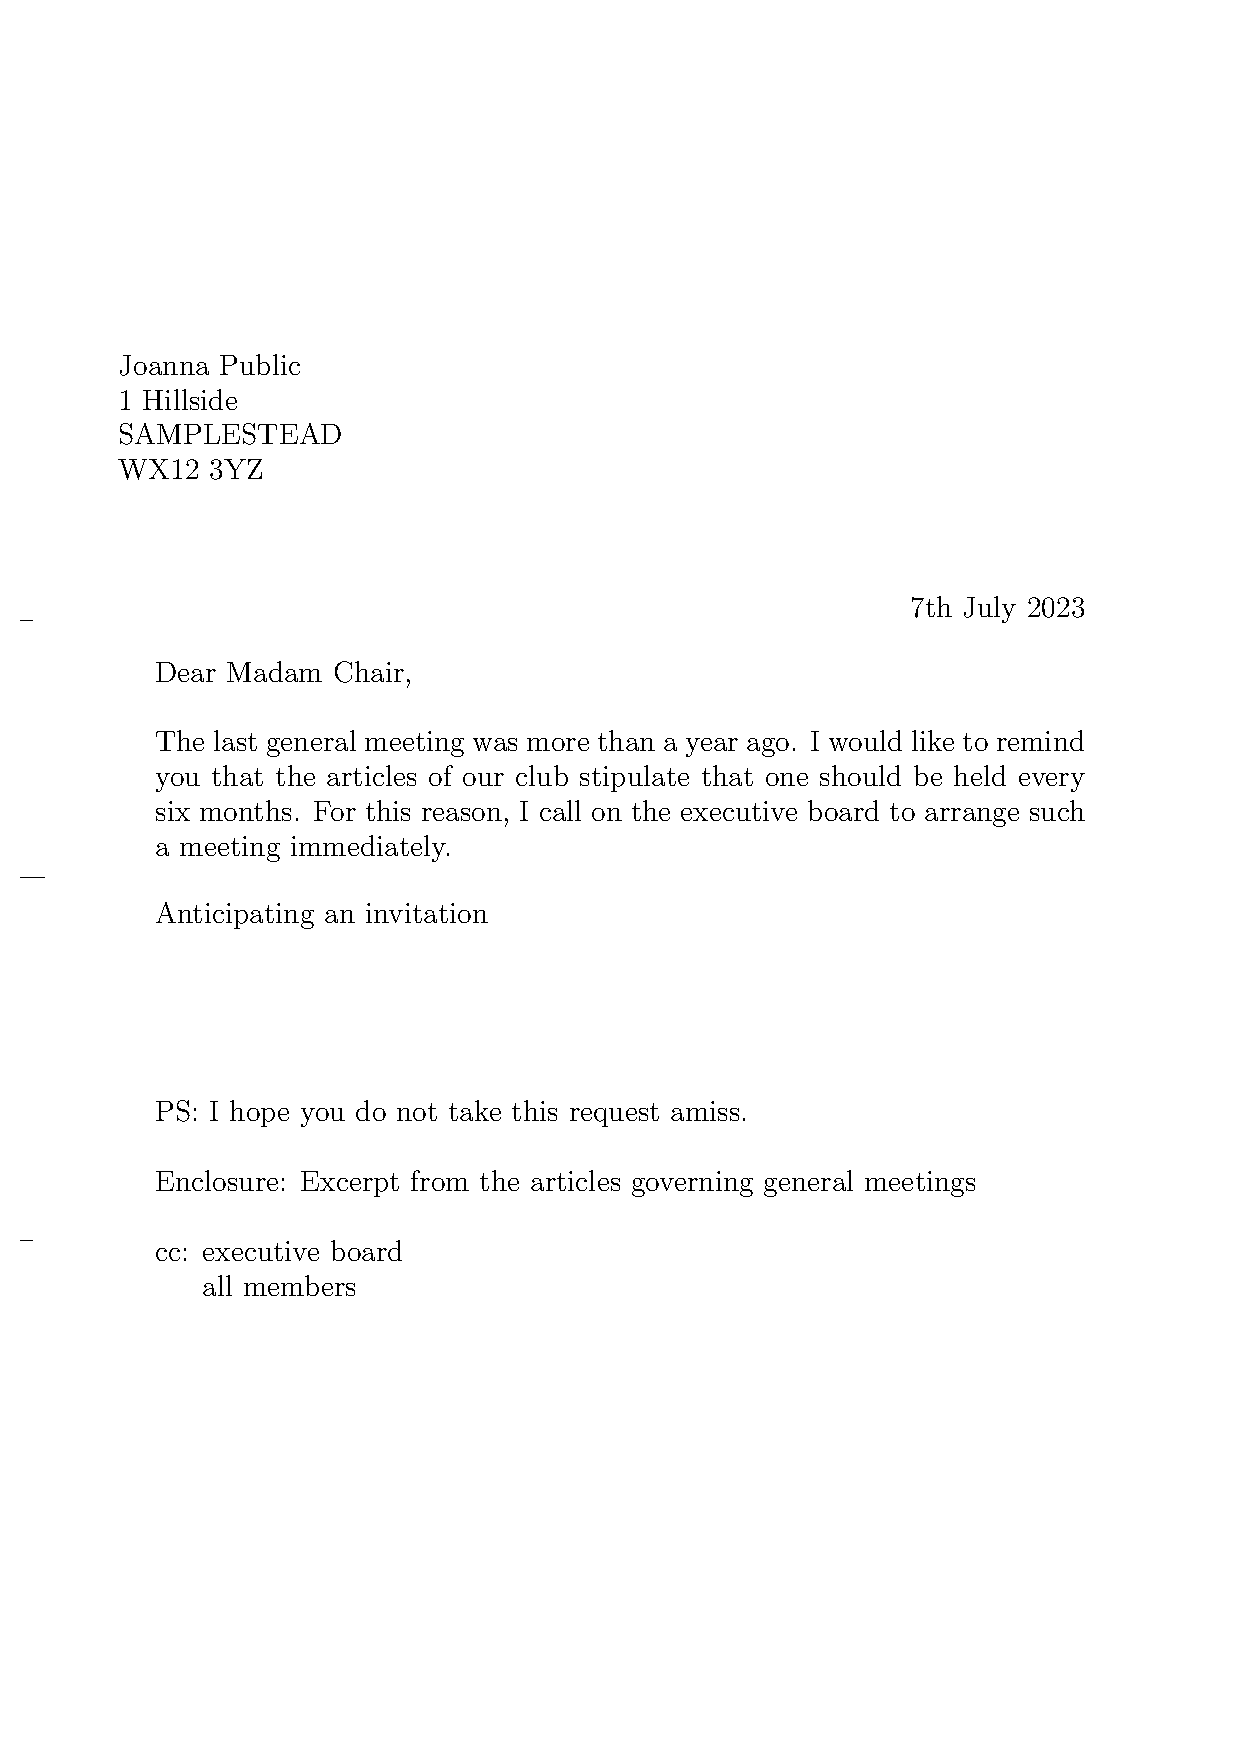
\includegraphics[width=.4\textwidth]{letter-example-05-en}}\quad
      \frame{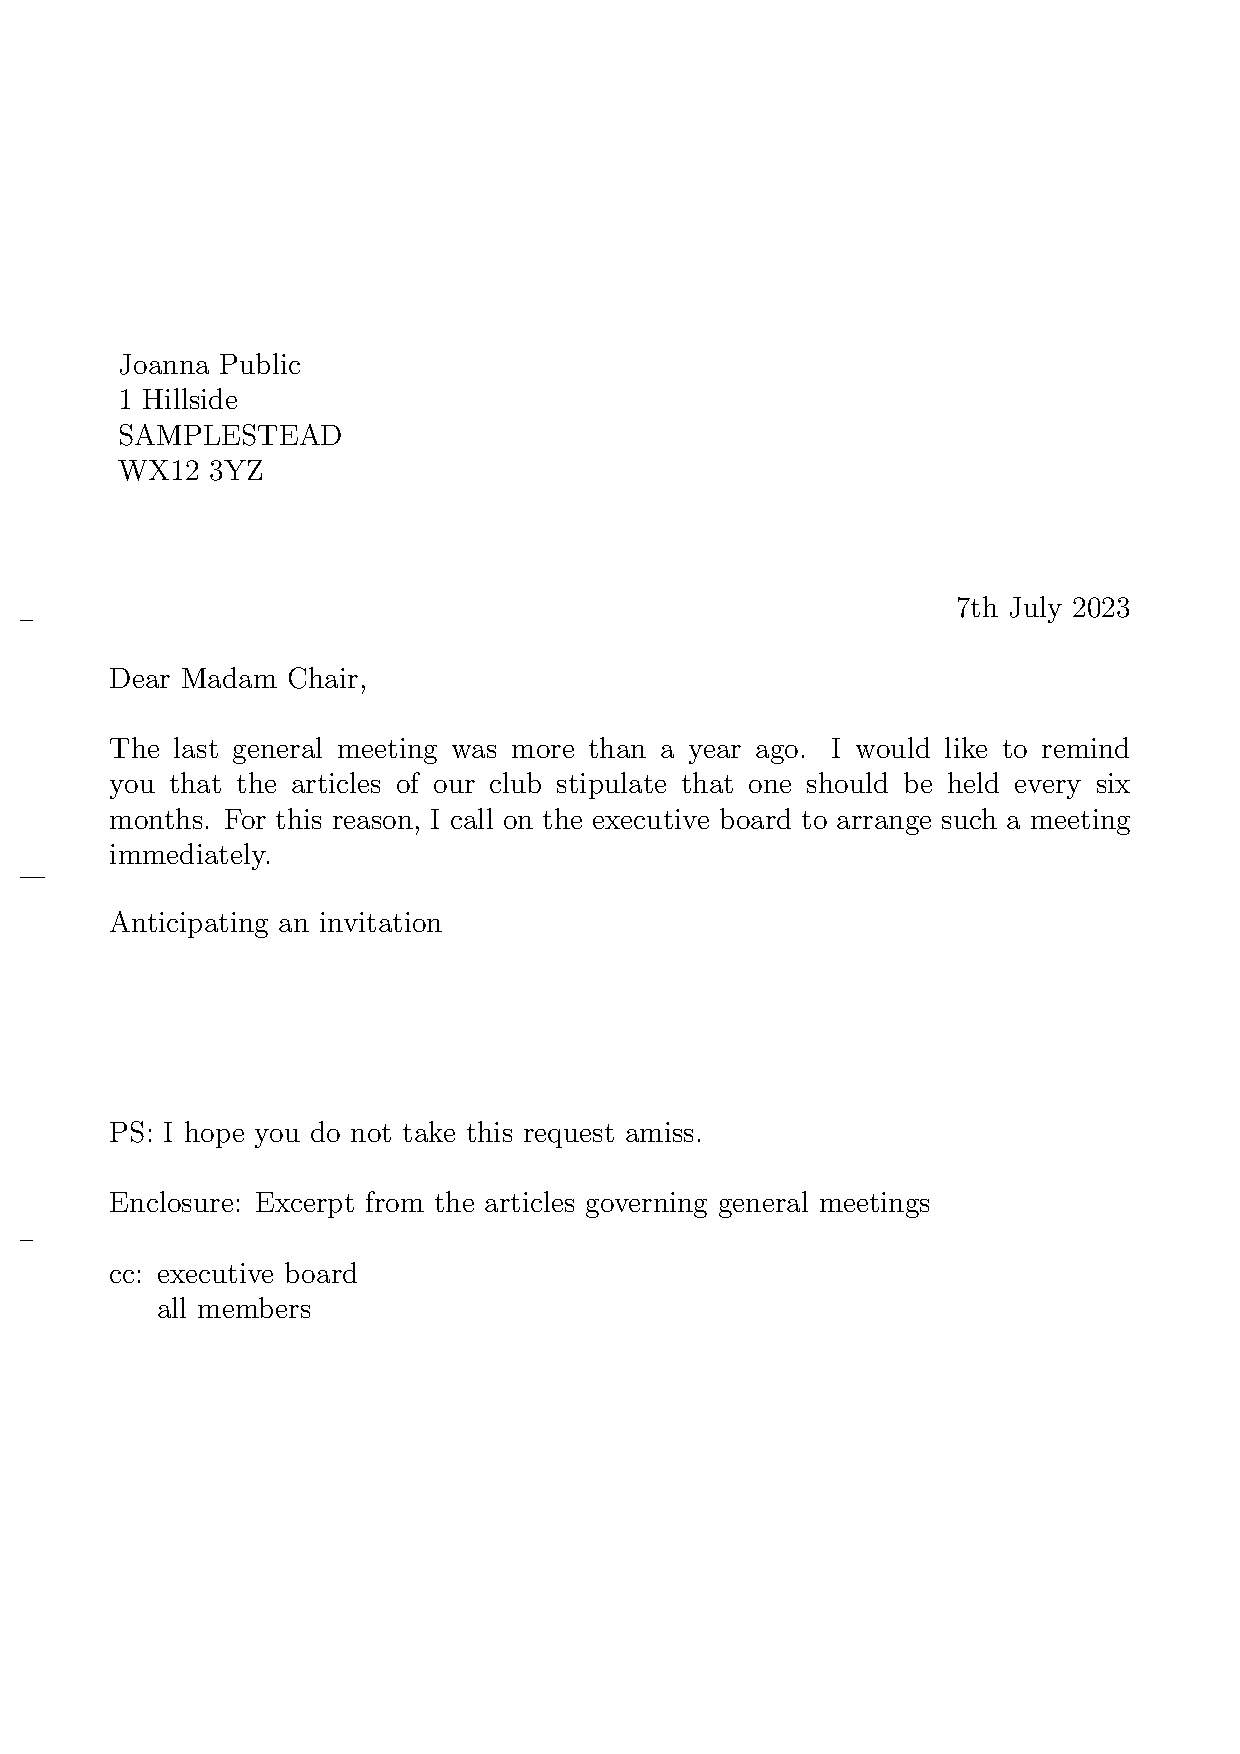
\includegraphics[width=.4\textwidth]{letter-example-06-en}}
      \caption[{Example: letter with address, salutation, text, closing phrase,
        postscript, enclosures, distribution list, and noxiously large font
        size}]
      {result of a short letter with recipient, opening, text, closing,
      postscript, enclosures, distribution list, and a noxiously large font
      (the date is set by default): in the left-hand version, the font size
      has been defined by the optional argument of
      \DescRef{\LabelBase.env.letter}; in the right-hand one, the optional
      argument of \DescRef{\LabelBase.cmd.documentclass} has been used}
      \label{fig:scrlttr2.letter-05-06}
    \end{figure}
  \end{Example}
  \ExampleEndFix
}{%
  \IfThisCommonLabelBase{maincls}{%
    \par
    \phantomsection\label{sec:\ThisCommonLabelBase.fontOptions.end}%
    The default for \Class{scrbook}, \Class{scrreprt}, and \Class{scrartcl} is
    \OptionValue{fontsize}{11pt}.\textnote{\KOMAScript{} vs. standard classes}
    In contrast, the default size in the standard classes is \Option{10pt}. 
    You may need to account for this difference if you switch from a standard 
    class to a \KOMAScript{} class\iffree{}{ or when using the
      \DescRef{maincls-experts.option.emulatestandardclasses}%
      \IndexOption{emulatestandardclasses} option}.%
  }{}%
}%
%
\EndIndexGroup
%
\EndIndexGroup


%%% Local Variables: 
%%% mode: latex
%%% TeX-master: "scrguide-en.tex"
%%% coding: utf-8
%%% ispell-local-dictionary: "en_GB"
%%% eval: (flyspell-mode 1)
%%% End: 
